
CMake's build process works in two steps, as shown in the following diagram. First, if it's invoked without any special flags, CMake scans the system for any usable toolchains during the configuration process and then decides what its output should be. The second step, which is when cmake -{}-build is invoked, is the actual compilation and building process:

\begin{center}
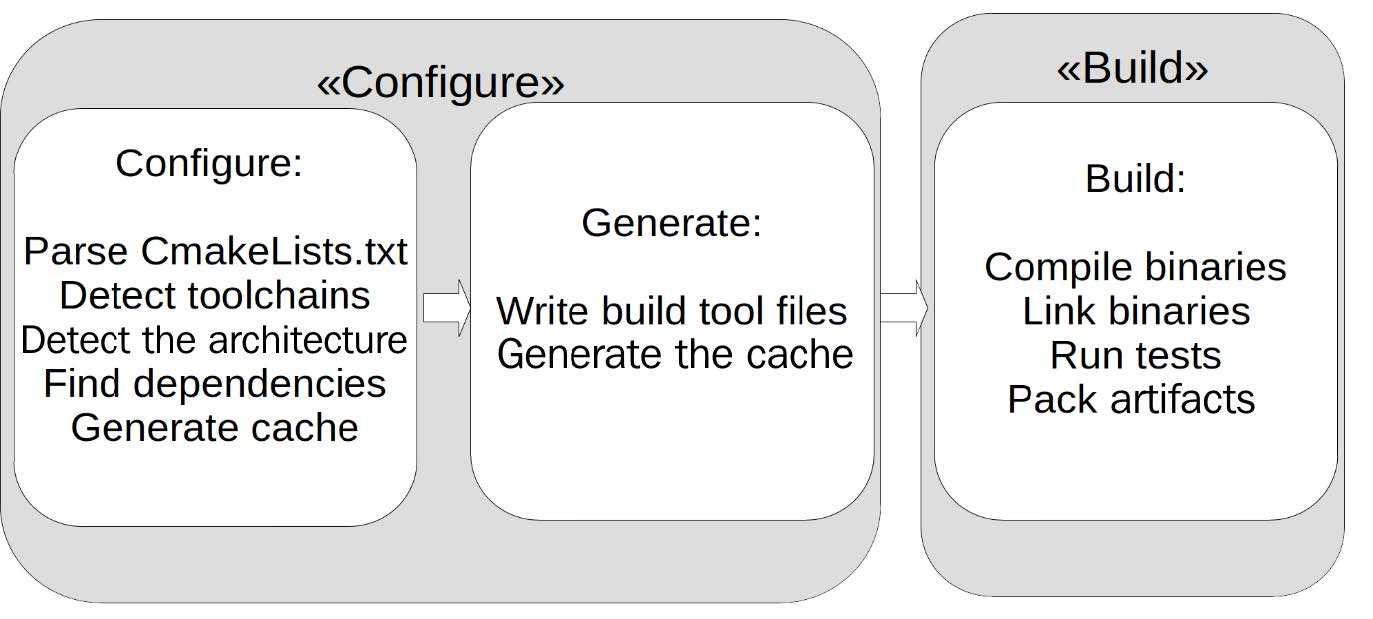
\includegraphics[width=1.\textwidth]{content/1/chapter1/images/3.jpg}\\
Figure 1.3 – CMake's two-stage build process
\end{center}

The standard output is Unix Makefiles unless the only detected compiler is Microsoft Visual Studio, in which case a Visual Studio solution (.sln) will be created. 

To change the generator, you can pass the -G option to CMake, like this:

\begin{tcblisting}{commandshell={}}
cmake .. -G Ninja
\end{tcblisting}

This will generate files to be used with Ninja (h\url{ttps://ninja-build.org/}), an alternative build generator. Many generators are available for CMake. A list of the ones that are supported natively can be found on CMake's website: \url{https://cmake.org/cmake/help/latest/manual/cmake-generators.7.html}.

There are two main types of generators – the ones where there are many Makefile flavors and Ninja generators, which are generally used from the command line, and the ones that create build files for an IDE such as Visual Studio or Xcode.

CMake addition differentiates between single-configuration generators and multiconfiguration generators. For single-configuration generators, the build files have to be rewritten each time the configuration is changed; multi-configuration build systems can manage different configurations without the need to regenerate. Although the examples in this book use single-configuration generators, they would also work on multiconfiguration generators. For most of the examples, the chosen generator is irrelevant; otherwise, it will be mentioned:

\begin{table}[H]
	\centering
	\begin{tabular}{|l|l|}
		\hline
		\textbf{生成器}                                                                                                                  &  \textbf{多配制}                                                            \\ \hline
		Makefile(all flavors)                                                                                                                                  &                                                                           No       \\  \hline
		Ninja              &                                                                                  No\\  \hline
		Ninja Multi-Config  &  Yes                                                                                \\ \hline
    Xcode              &                                                                                  Yes\\  \hline
    Visual Studio              &                                                                                  Yes\\  \hline
	\end{tabular}
\end{table}

In addition, there are extra generators that use a normal generator but also produce project information for an editor or IDE, such as Sublime Text 2, Kate Editor, Code::Blocks, and Eclipse. For each, you can select whether the editor should use Make or Ninja to internally build the application.

After the call, CMake will create a lot of files in the build folder, with the most notable being the CMakeCache.txt file. This is where all the detected configurations are stored. Note that when you're using cmake-gui, the first step is split into configuring the project and generating the build file. However, when it's run from the command line, the steps are merged into one. Once configured, all the build commands are executed from the build folder.

\subsubsubsection{1.5.1\hspace{0.2cm}Source folders and build folders}

In CMake, two logical folders exist. One is the source folder, which contains a hierarchical set of projects, while the other is a build folder, which contains the build instructions, cache, and all the generated binaries and artifacts.

The root of the source folder is wherever the top CMakeLists.txt file is located. The build folder can be placed inside the source folder, but some people prefer to have it in another location. Both are fine; note that for the examples in this book, we decided to keep the build folder inside the source folder. The build folder is often called just build, but it can take any name, including prefixes and suffixes for different platforms. When using a build folder inside the source tree, it is a good idea to add it to .gitignore so that it does not get checked in accidentally.

When configuring a CMake project, the project and folder structure of the source folder is recreated inside the build folder so that all the build artifacts are in the same position. In each mapped folder, there is a subfolder called CMakeFiles that contains all the information that's generated by CMake's configuration step.

The following code shows an example structure for a CMake project:

\begin{tcblisting}{commandshell={}}
.
├── chapter_1
│      ├── CMakeLists.txt
│      └── src
│            └── main.cpp
├── CMakeLists.txt
\end{tcblisting}

When you execute the CMake configuration, the file  structure of the CMake project is mapped into the build folder. Each folder containing a CMakeLists.txt file will be mapped and a subfolder called CMakeFiles will be created, which contains the information that's used by CMake for building:

\begin{tcblisting}{commandshell={}}
├── build
│     ├── chapter_1
│     │      └── CMakeFiles
│     └── CMakeFiles
\end{tcblisting}

So far, we have used existing projects to learn about the CMake build process. We learned about the configuration and the build step, as well as generators, and that we need CMakeLists.txt files to pass the necessary information to CMake. So, let's go a step further and see what the CMakeLists.txt files look like and how the CMake language works.























